\documentclass[paper=a4,fontsize=10pt,jafontsize=10pt,line_length=44zw,number_of_lines=46]{jlreq}
\usepackage{amsmath,amssymb,graphicx,booktabs,multirow,siunitx,xcolor}
\usepackage[hidelinks]{hyperref}
\sisetup{detect-all}
\newcommand{\tauh}{\tau_{\mathrm{h}}}
\newcommand{\taul}{\tau_{\ell}}
\newcommand{\bbtt}{b\bar b\tau^+\tau^-}
\newcommand{\abinv}{\,\mathrm{ab}^{-1}}
\newcommand{\fbinv}{\,\mathrm{fb}^{-1}}
\newcommand{\hvec}{\boldsymbol{h}}

\title{$\tau$レプトンのスピンと寿命の情報によるHL-LHCでの\\$HH\to\bbtt$探索感度の改善の見積もり}
\author{（著者名）\\（所属）}
\date{2026年10月}

\begin{document}
\maketitle

\begin{abstract}
高輝度LHC（HL-LHC，$\sqrt{s}=14$\,TeV，$3\abinv$）で標準模型のHiggs粒子対生成$HH$を観測できるかどうかは，Higgs自己結合の測定にとって最重要の課題の一つであり，ATLASの最新の投影では期待有意度が$4.3\sigma$（$\bbtt$チャンネルは$3.5\sigma$）である．本論文では，$\tau$レプトンのスピンと寿命の情報を$\bbtt$探索に加えることで，この有意度がどこまで改善しうるかを見積もる．スピンの情報は，一次頂点を基準にした衝突径数（impact parameter, IP）と二次頂点を$\tau$の局所座標で表して$\tau$の偏極計ベクトルを回帰する手法（tauspin）で得る．寿命の情報は，同じIPをレプトンに適用し，$\tau$崩壊由来のレプトンと$W$崩壊由来の即発レプトンを区別することで得る．14\,TeVの事象生成とATLASの完全シミュレーションに較正した検出器応答を用い，スピン無偏極で崩壊させた試料の厳密な再重み付けとAsimov尤度によって評価した．$\tauh\tauh$チャンネルの信号らしさが最も高い領域では，スピン情報による有意度の改善は$+2.4\%$にとどまり（崩壊生成物から偏極計が正確に分かる理想的な場合でも$+12.6\%$），背景の大半が信号と同じスピン状態をもつ単一Higgs粒子と，スピンでの分離が本質的に弱い$Z$+重フレーバーで占められていることがその原因である．一方，$\taul\tauh$チャンネルでは，レプトンの寿命情報によって信号らしさが最も高い領域の有意度が$1.13$〜$1.21$倍に改善する（ATLAS Run~2の背景組成，現実的な分解能，非即発レプトンの混入，IP分布の幅の不定性を含む全ての変種での範囲）．両者をATLASのHL-LHC投影に例示的に換算すると，$\bbtt$チャンネルは$3.5\sigma$から$3.59$〜$3.80\sigma$，ATLASの$HH$結合は$4.3\sigma$から$4.38$〜$4.54\sigma$，ATLAS+CMSは$7.2\sigma$から$7.29$〜$7.49\sigma$となる．改善は控えめだが，レプトンの寿命情報は著者らの知る限り既存の$HH$解析で使われていない．また，ATLASの信号領域のレプトンに$d_0$有意度の要求が課されているかは確認できていないが，課されている場合には，それを外すことでさらに大きな改善の余地がある．
\end{abstract}

\section{序論}

Higgs粒子の自己結合$\lambda_{HHH}$は，Higgsポテンシャルの形を直接に決める量であり，電弱対称性の破れの機構を検証するうえで中心的な役割を果たす．LHCでは，グルーオン融合による$HH$対生成の断面積が三点自己結合に依存することを利用して測定が行われ，標準模型（SM）の値で規格化した$\kappa_\lambda=\lambda_{HHH}/\lambda_{HHH}^{\mathrm{SM}}$が制限されている\cite{Glover:1987nx,Dawson:1998py}．$HH$のSM断面積は$\sqrt s=14$\,TeVで約$37$\,fbと小さく，HL-LHCの$3\abinv$をもってしても観測は容易ではない．ATLASの最新の投影では，$b\bar b\gamma\gamma$，$\bbtt$，$b\bar bb\bar b$などを結合した期待有意度は$4.3\sigma$であり，そのうち$\bbtt$チャンネルは$3.5\sigma$（$\tauh\tauh$ $3.1\sigma$，$\taul\tauh$ $1.8\sigma$）を担う\cite{ATL-PHYS-PUB-2025-018,ATL-PHYS-PUB-2024-016}．ATLASとCMSを合わせると$7.2\sigma$と見込まれている\cite{ATL-PHYS-PUB-2025-018}．$5\sigma$の観測に向けて，既存の解析で使われていない情報を加える余地を探ることには意味がある．

$\bbtt$チャンネルの背景は，$t\bar t$，$Z(\to\tau\tau)$+重フレーバー（$Z$+HF），単一Higgs粒子（$ZH$，$t\bar tH$など），およびジェットが$\tauh$と誤認されるfake背景からなる\cite{ATLAS:2022xzm}．信号の$H\to\tau\tau$では二つの$\tau$のスピンがCP偶のスカラーに特有の形で相関し，$W\to\tau\nu$由来の$\tau$は完全に縦偏極し，$Z\to\tau\tau$では縦方向の相関が逆符号になる．このスピン構造の違いは原理的に背景の除去に使える．ただし，ニュートリノが失われるため，$\tau$のスピン情報を担う偏極計ベクトル$\hvec$を測定量から正確に復元することはできない．

著者らは先行研究（tauspin，未発表）で，一次頂点（PV）を基準にした衝突径数（IP）と二次頂点（SV）を$\tau$の局所座標で表し，偏極計ベクトルそのものを機械学習で回帰する手法を開発した．ATLASの完全シミュレーションで，同じ質量の$H$と$Z$を$\tau\tau$のスピンだけで区別する性能がAUC（ROC曲線の下の面積）で$0.626$（正確な偏極計を使った上限が約$0.72$〜$0.73$）に達し，IPが可視粒子と欠損運動量だけでは決まらない$\tau$の方位角を約$2$\,mradの精度で測ることを示した．本論文では，この手法を$HH\to\bbtt$探索に応用し，期待有意度がどこまで改善するかを定量的に評価する．

評価は二つの経路で行う．第一は，$\tauh\tauh$チャンネルでの$\tau$対のスピン状態による背景除去である．第二は，tauspinの中心にあるPV基準のIPをレプトンへ広げ，$\taul\tauh$チャンネルで$\tau$崩壊由来のレプトン（信号，$Z\to\tau\tau$，$H\to\tau\tau$）と$W$崩壊由来の即発レプトン（$t\bar t$，単一top，fake背景の大半）を区別することである．後者はスピンではなく$\tau$の寿命の情報であり，ATLASが$t\bar t$事象でミューオンの$|d_0|$を使って$W\to\tau\nu$と$W\to\mu\nu$の分岐比の比$R(\tau/\mu)$を測定した手法\cite{ATLAS:2020xea}と同じ物理に基づく．著者らの知る限り，この寿命情報を$HH\to\bbtt$の分類に使った例はない．

本論文の構成は以下のとおりである．第\ref{sec:tauspin}節でtauspinの手法とレプトンへの拡張を述べる．第\ref{sec:sim}節で事象生成と検出器応答の模擬を，第\ref{sec:stat}節でスピン仮説の再重み付けと統計手法を説明する．第\ref{sec:hadhad}節と第\ref{sec:lephad}節でそれぞれ$\tauh\tauh$と$\taul\tauh$の結果を示し，第\ref{sec:proj}節でATLASのHL-LHC投影への換算を行う．第\ref{sec:disc}節で限界と今後の課題を議論し，第\ref{sec:concl}節でまとめる．

\section{tauspinの手法とレプトンへの拡張}\label{sec:tauspin}

\subsection{$\tau$対のスピン密度と偏極計ベクトル}

$\tau$の崩壊は，$\tau$静止系での偏極計ベクトル$\hvec$（$|\hvec|\le 1$）を通じてのみスピンに依存する．二つの$\tau$の崩壊生成物の分布は
\begin{equation}
  \frac{d\Gamma}{d\Phi}\propto 1+\boldsymbol{B}^-\!\cdot\hvec^-+\boldsymbol{B}^+\!\cdot\hvec^+ +\sum_{ij}C_{ij}\,h^-_ih^+_j
  \label{eq:rho}
\end{equation}
と書ける．$\boldsymbol B^\pm$は各$\tau$の偏極，$C_{ij}$はスピン相関行列である．各$\tau$の運動量方向を$k$，それとビーム軸の張る面に垂直な方向を$n$，残りを$r$とする局所基底を取ると，本論文の符号規約では，CP偶のHiggs粒子は$\boldsymbol B^\pm=0$，$C=\mathrm{diag}(1,1,-1)$（$n,r,k$の順），$Z$は$C_{kk}=+1$，$\tau$の縦偏極$P_\tau=-0.147$，$W$由来の$\tau$は$1-h_k$で表される完全偏極，fake $\tau$はスピン構造なし，となる．偏極計を実装した崩壊モードは$\pi$，$\rho$，$\pi2\pi^0$，$3\pi$の4つで，$\tau$の1本当たり$\tau$のハドロン崩壊の$84\%$，$\tau$対の両側では$71\%$を覆う．$3\pi$の偏極計はPythia~8が用いるCLEOのハドロン流\cite{Bierlich:2022pfr}を移植して計算した．

\subsection{回帰による偏極計の推定}

tauspinは，各$\tau$の可視崩壊生成物（荷電トラックと$\pi^0$クラスターの運動量），先頭トラックのPV基準IPベクトル，三本トラック崩壊のSVの方向，欠損横運動量の射影を，$\tau$の局所基底$(n,r,k)$で表した入力とし，二つの$\tau$の偏極計$\hvec^\pm$と積$h^-_ih^+_j$を多層パーセプトロンで回帰する．学習には，スピンの情報が質量から漏れないよう，Pythia内部で生成した$H(125)$+ジェットと，$Z$の質量を$125$\,GeVに置き換えた$Z$+ジェット（結合とスピン構造は$Z$のまま）を同数用いる．

本研究の模擬検出器（第\ref{sec:sim}節）で学習し直した回帰器は，取り置いた等質量$H/Z(125)$事象で，回帰値と真の偏極計の相関が横成分$0.61/0.62$，縦成分$0.73$（ATLAS完全シミュレーションで$0.62/0.58/0.765$），回帰値から作る固定した読み出しの$H/Z$ AUCが$0.627$（同$0.626$），正確な偏極計の尤度比のAUCが$0.730$（同$0.719$〜$0.729$）となり，tauspinのATLAS完全シミュレーションでの到達点を再現した（図\ref{fig:closure_hz}）．ただし応答の較正には同じATLAS検証データを使っているので，これは独立な検出器検証ではなく，模擬をtauspinの実力に合わせたことの確認である．

\begin{figure}[t]
  \centering
  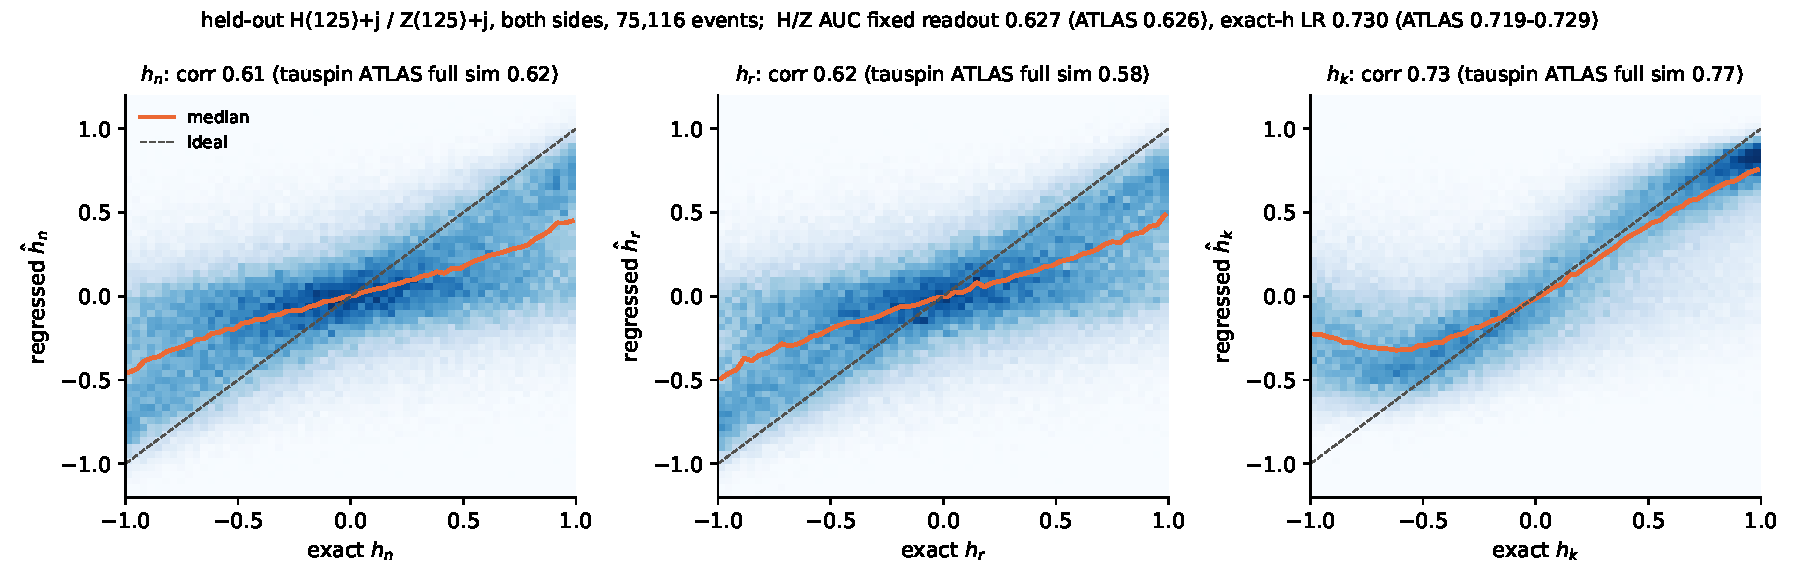
\includegraphics[width=\linewidth]{figures/phase2_closure_h_regression.pdf}
  \caption{模擬検出器と回帰器がtauspinのATLAS完全シミュレーションの性能を再現していることの確認．等質量$H/Z(125)$+ジェットの取り置き試料での，偏極計の各成分の回帰値と真値の関係と，$H/Z$の分離．}
  \label{fig:closure_hz}
\end{figure}

\subsection{レプトンへの拡張：$\tau$の寿命の情報}

$\tau$の固有崩壊長は$c\tau=87\,\mu$mであり，崩壊で生じたレプトンの飛跡はPVを通らない．$\tau$がPVから$\boldsymbol L$だけ飛んで崩壊したとき，レプトンの方向を$\hat k$とすると，IPベクトルは$\boldsymbol L-(\boldsymbol L\cdot\hat k)\hat k$であり，その大きさは$\tau$の運動量によらず$c\tau$程度になる．一方，$W$や$Z$の崩壊で直接生じたレプトンのIPは0であり，測定値は分解能だけで決まる．tauspinでハドロン側の$\tau$に用いたPV基準のIPを，そのままレプトンに適用すれば，レプトンの起源を区別できる．ATLASの$R(\tau/\mu)$測定\cite{ATLAS:2020xea}は，$t\bar t$事象のミューオンの$|d_0|$と$p_T$の分布でこの区別を行い，$R(\tau/\mu)=0.992\pm0.013$を得た．本研究では，レプトンのIPを$|d_0|/\sigma(d_0)$，$z_0\sin\theta$の有意度，およびtauspinと同じ局所基底での3次元ベクトルとして分類器に加える．

\section{事象生成と検出器応答の模擬}\label{sec:sim}

\subsection{事象生成}

全ての試料は$\sqrt s=14$\,TeVで，MadGraph5\_aMC@NLO~3.5.9\cite{Alwall:2014hca}による最低次（LO）のハード過程と，Pythia~8.315\cite{Bierlich:2022pfr}によるパートンシャワー・ハドロン化・$\tau$崩壊で作った（表\ref{tab:samples}）．$\tau$の崩壊はPythiaに任せ，スピン相関は母粒子から引き継がせる．ここで一つ技術的な注意がある．MadGraphの出力するLes Houches事象（LHE）ファイルはHiggs粒子のヘリシティ（SPINUP）を0と書くため，Pythiaの既定の\texttt{TauDecays:mode = 1}では外部ヘリシティの経路に入り，$H\to\tau\tau$のスピン相関が失われる．本研究では\texttt{TauDecays:mode = 4}（内部の行列要素のみ）を用い，$HH$で$C\approx\mathrm{diag}(0.82,0.94,-0.95)\pm0.1$，$t\bar t$の$W$由来$\tau$で$\langle h_k\rangle=-0.33$（$P\approx-1$に相当），$Z\to\tau\tau$で$C_{kk}=+1.01$，$P_\tau\approx-0.15$となることを確かめた．MadGraphとPythiaで$HH\to\bbtt$を作る他の研究でも同じことが起こりうる．

スピン仮説の再重み付け（第\ref{sec:stat}節）のため，同じ$HH$のLHEを$\tau$を無偏極・無相関に崩壊させて（\texttt{TauDecays:mode = 3}，偏極0）シャワーした「スピン平坦」試料も作った．この試料の生成スピン密度は1なので，任意のスピン仮説$X$への重みは$\rho_X(\hvec)$そのもの（有界）になる．$8000$事象で$C\approx0$，$\langle\hvec\rangle\approx0$を確認した．

\begin{table}[t]
  \centering
  \caption{用いた試料．断面積は規格化に用いた値で，崩壊分岐比を含む．$t\bar t$は$984.5$\,pb（NNLO+NNLL），$tW$は両電荷で$84$\,pb，$W$の分岐比は$e$ $0.1071$，$\mu$ $0.1063$，$\tau$ $0.1125$，ハドロン$0.6741$とした．$Z+b\bar b$は生成器の値に$1.3$を掛けた．}
  \label{tab:samples}
  \small
  \begin{tabular}{llr}
    \toprule
    過程 & 用途 & 生成事象数 \\
    \midrule
    $gg\to HH$（$H\to b\bar b$，$H\to\tau\tau$；$\sigma=36.69$\,fb） & 信号（スピン相関あり／スピン平坦） & $2.0\times10^6$ ずつ \\
    $t\bar t\to b\tau\nu\,b\tau\nu$ & 背景 & $2.0\times10^6$ \\
    $t\bar t\to b\tau\nu\,bjj$ & fake背景（$\tau$側は真の$\tau$） & $1.0\times10^6$ \\
    $t\bar t\to b\ell\nu\,b\tau\nu$（$\ell=e,\mu$） & 背景（$\taul\tauh$用） & $4.0\times10^6$ \\
    $t\bar t\to b\ell\nu\,bjj$ & fake背景（$\taul\tauh$用） & $3.0\times10^6$ \\
    $tW$（両$W\to\ell/\tau$） & 単一top & $1.0\times10^6$ \\
    $tW$（片方$W\to\ell/\tau$，他方$W\to jj$） & fake背景 & $2.0\times10^6$ \\
    $Z(\to\tau\tau)b\bar b$ & $Z$+HF & $1.5\times10^6$ \\
    $ZH$（$Z\to b\bar b$，$H\to\tau\tau$） & 単一Higgs & $3\times10^5$ \\
    $t\bar tH$（$H\to\tau\tau$） & 単一Higgs & $3\times10^5$ \\
    $H(125)$+jet，$Z(125)$+jet（Pythia，$\hat p_T>40$\,GeV） & 回帰器の学習 & $3\times10^6$ ずつ \\
    \bottomrule
  \end{tabular}
\end{table}

\subsection{検出器応答}

検出器応答はパラメトリックに模擬し，その値はtauspinのATLAS完全シミュレーション検証試料（$59{,}390$事象）で測ったものに合わせた．
\begin{itemize}
  \item $\pi^0$クラスターのエネルギー分解能$\sigma/E=0.95/\sqrt E\oplus0.06\oplus3.2/E$，角度分解能$0.06/\sqrt E\oplus0.003$\,rad．
  \item 荷電トラックの運動量分解能$\sigma(p_T)/p_T=0.02\oplus4\times10^{-4}p_T$．
  \item 崩壊モードの移行：$\rho$で$\pi^0$を失う確率$10\%$，$\pi$に偽の$\pi^0$が付く確率$8.7\%$など．
  \item IP：$d_0$は$10\oplus150/p_T\,\mu$m，$z_0$は$20\oplus300/p_T\,\mu$m．SV：横$10\,\mu$m，飛行方向$250\,\mu$m．
  \item 欠損横運動量：真値から各物体の測定誤差を引き，成分ごとに$18$\,GeVのソフト項を加える．
  \item ジェット：$\sigma/E=0.8/\sqrt E\oplus0.05$，$b$タグ効率は$b$ $77\%$，$c$ $20\%$，軽いクォーク$1\%$．
  \item $\tau$の識別効率：1本トラック$0.85$，3本トラック$0.75$．fake $\tau$はジェットの芯の構成粒子から作り，fake因子（1本$10^{-2}$，3本$3\times10^{-3}$）を事象の重みとする．
\end{itemize}
レプトン（$e$，$\mu$）の識別・孤立の効率は$0.90$，$0.95$とし，運動量分解能はミューオン$2\%\oplus0.03\%\,p_T$，電子$1.5\%\oplus10\%/\sqrt E$とした．レプトンのIPの分解能は，名目値として$\tau$のトラックと同じ$d_0$分解能（電子は制動放射のため$1.2$倍）に，$2\%$の割合で4倍幅の裾を加えた．現実的な模型として，ビームスポットの$10\,\mu$mを二乗和で加え，$(1+0.2|\eta|)$の$\eta$依存性と電子の追加の裾（$7\%$，4倍幅）を入れたものも用いる．PVは原点に固定した．

\subsection{事象選別と質量再構成}

$\tauh\tauh$チャンネルでは，ATLASのRun~2解析\cite{ATLAS:2022xzm}に倣い，$p_T>40$，$30$\,GeVで反対電荷の二つの$\tauh$，ちょうど2本の$b$タグジェット（$p_T>45$，$20$\,GeV），即発レプトンの不在を要求する．$\taul\tauh$チャンネルでは，ちょうど1個のレプトン（$e$: $p_T>18$，$\mu$: $p_T>15$\,GeV）と反対電荷の$\tauh$（$|\eta|<2.3$）を要求し，レプトンの$p_T$が$27$\,GeVを超える事象を単一レプトン・トリガー（SLT）の領域（$\tauh$の$p_T>20$\,GeV），それ以外をレプトン＋$\tauh$トリガー（LTT）の領域（$\tauh$の$p_T>30$\,GeV）に分ける．いずれも$m_{bb}<150$\,GeV，$m_{\tau\tau}^{\mathrm{MMC}}>60$\,GeVを課す．

$\tau\tau$の不変質量は，tauspinで実装したMissing Mass Calculator（MMC）\cite{Elagin:2010aw}で求める．$\taul\tauh$用には，レプトン側の二つのニュートリノの不変質量$m_{\nu\nu}$を$[0,m_\tau]$で一様にサンプリングし，質量殻条件を$m_\tau^2=m_{\mathrm{vis}}^2+m_{\nu\nu}^2+2(E_{\mathrm{vis}}E_\nu-\boldsymbol p_{\mathrm{vis}}\!\cdot\boldsymbol p_\nu)$に拡張した．$HH$の$\taul\tauh$で中央値$126$\,GeV，成功率$98\%$である．

\section{スピン仮説の再重み付けと統計手法}\label{sec:stat}

\subsection{スピン平坦試料の再重み付け}

背景のMC統計で信号的な領域を直接評価することはできない（$t\bar t$を信号らしさが最も高い領域まで落とすには$10^{-4}$程度の除去が必要で，その領域に残るMC事象は0〜2個である）．そこで，$\tauh\tauh$チャンネルでは，スピン平坦$HH$試料を各スピン仮説（$H$，$Z$，$W$対，スピンなし$U$）へ$\rho_X(\hvec)$で再重み付けし，$HH$と同じ運動学の上でスピン判別量の分布を作る．偏極計が片側だけで定義される事象には周辺密度（$Z$: $1-0.147h_k$，$W$: $1-h_k$，$H$と$U$: 1）を用いる．スピン判別量は，回帰した$\hat{\hvec}^\pm$，積，再構成モードを入力とする多クラス分類器（2分割の交差学習）である．

この方法の妥当性は，スピン平坦試料を$H$仮説へ重み付けしたものと，同じLHEをスピン相関付きでシャワーした実際の$HH$とを比べることで検証した（図\ref{fig:hh_templates}(a)）．判別量の分布の$\chi^2/\mathrm{ndf}$は$12.9/20$，運動学的に信号らしさが最も高い$20\%$の領域で，学習に使わなかった事象での評価で$16.0/15$である．正確な偏極計のモーメントで見ると，重み付け後の横相関（$1.046,1.053$）は実際の$HH$（$0.945,0.983$）よりやや大きい．これは$\tau$のQED放射による方向の回転を理想的な$\rho_H$で表せないためと考えられる．横相関を$0.92$倍した変種でも，回帰によるスピン利得は変わらない（$1.0231$）．

\subsection{背景組成と尤度}

$\tauh\tauh$の評価は，ATLAS Run~2解析の信号らしさが最も高いビン\cite{ATLAS:2022xzm}の組成を$3\abinv$と14\,TeVの断面積比で換算したもの（$S=40.8$，$B=155$；背景の$28\%$が単一Higgs，$44\%$が$Z$+HF，$16\%$がtop，残りがfakeなど）に，各成分のスピン判別量の分布を掛けて行う．期待有意度は，$\mu=0$の仮説に対するAsimovデータの発見検定統計量$q_0$\cite{Cowan:2010js}で求め，背景の規格化に$Z$+HF $10\%$，top $10\%$，fake $20\%$，単一Higgs $15\%$のガウス型の局外パラメータ（nuisance parameter）を入れてプロファイルする．スピン判別量のテンプレートの仮説間の差には，$25\%$の形状の局外パラメータを加えた変種も評価する．利得はスピン判別量でビンを分割したときとしないときの有意度の比$R=Z_{\mathrm{split}}/Z_{\mathrm{bin}}$で表す．

ATLASの解析は運動学的なブースト決定木（BDT）の出力でビンを作っている．スピン情報がBDTと二重に数えられないことを確かめるため，運動学的な分類器$K$の出力で信号効率$100/50/20/5\%$の領域を切り，その中で「運動学のみ」「運動学＋スピン」の分類器の増分も評価した．

\section{$\tauh\tauh$チャンネル：スピン情報による利得}\label{sec:hadhad}

\begin{figure}[t]
  \centering
  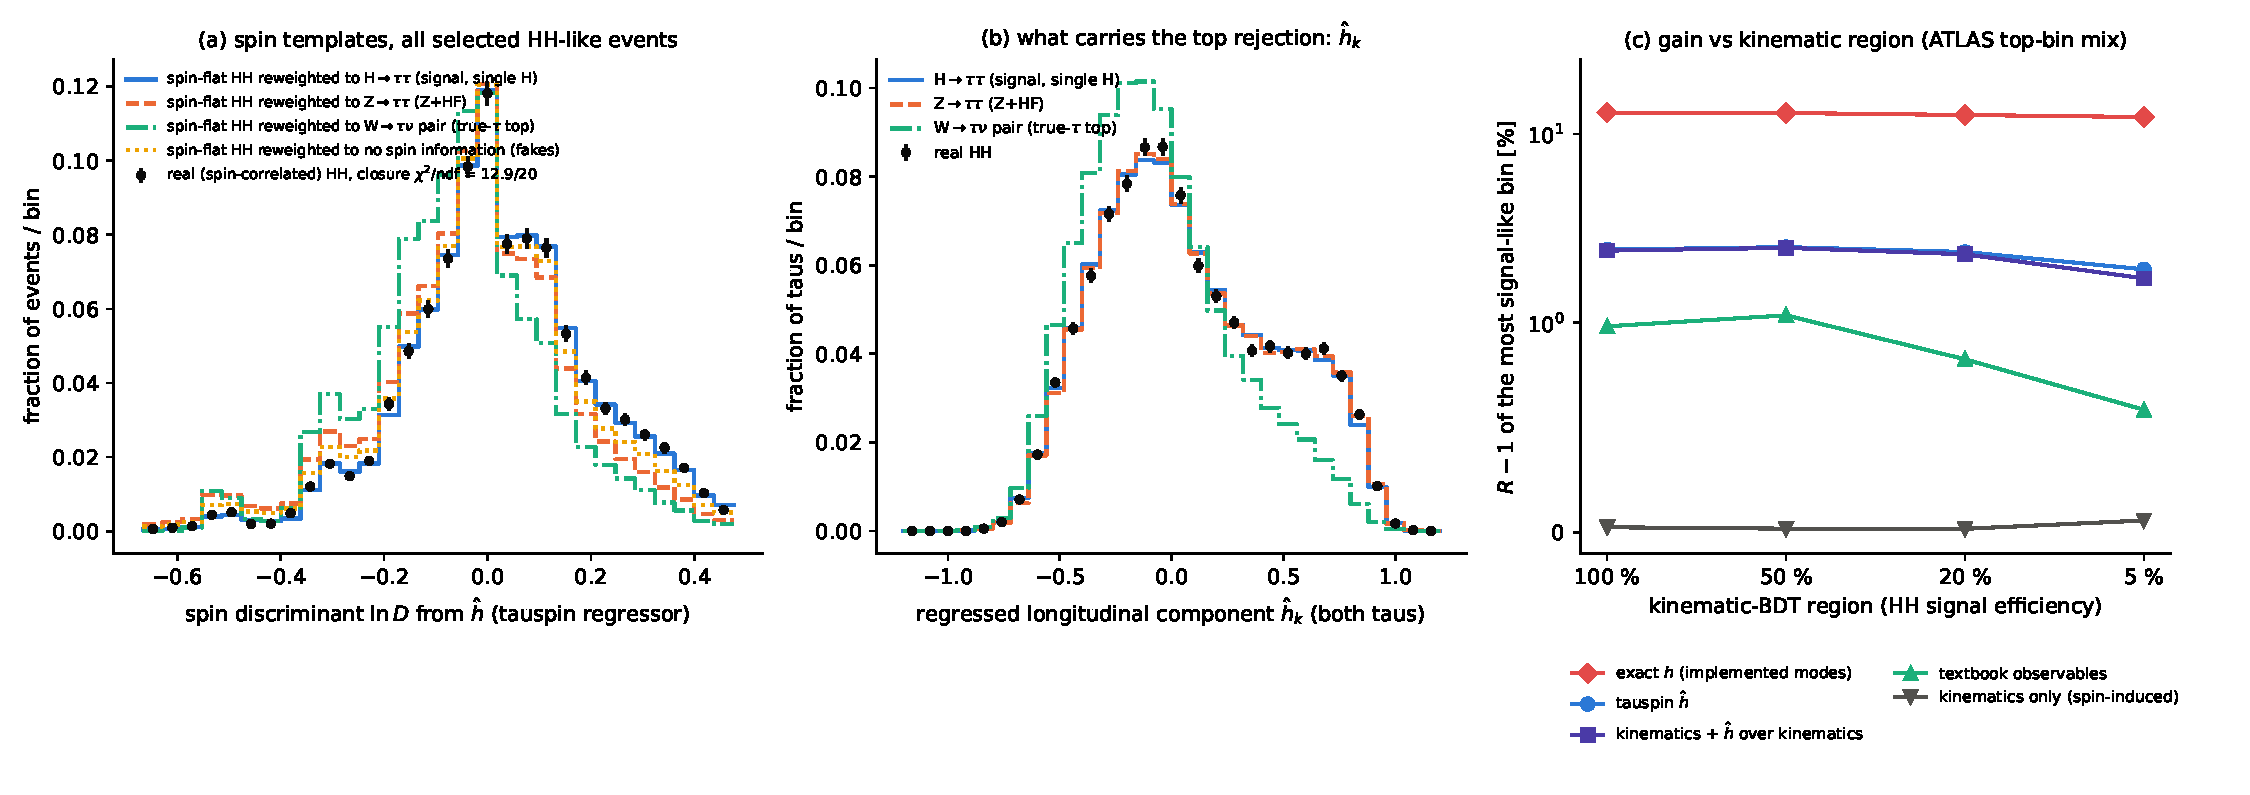
\includegraphics[width=\linewidth]{figures/v2_spin_templates_closure_region.pdf}
  \caption{(a) スピン平坦$HH$を各スピン仮説へ重み付けしたときの，回帰した偏極計から作るスピン判別量の分布．黒点は実際のスピン相関付き$HH$で，$H$仮説を再現する．(b) $\tau$1本の縦成分$\hat h_k$．$W$由来の$\tau$（top）だけが負側へずれ，$H$と$Z$はほぼ重なる．(c) 運動学的BDTの領域ごとの利得$R-1$．}
  \label{fig:hh_templates}
\end{figure}

表\ref{tab:hadhad}に結果をまとめる．tauspin水準の回帰による利得は，運動学的に信号らしさが最も高い$20\%$の領域で$R=1.0237$（分類器の学習し直しによるばらつき$\pm0.0009$）であり，$25\%$の形状の局外パラメータを入れても$1.0233$である．$Z$の横相関（$C_{nn}=+0.49$，$C_{rr}=-0.46$）を入れると$1.0243$（正確な偏極計で$1.130$）で，ほとんど変わらない．$\Upsilon$（荷電と中性のエネルギー非対称）やエネルギー分率などの教科書的な観測量では$1.008$にとどまる．崩壊生成物から偏極計を正確に知っている理想的な場合でも，実装した4つの崩壊モードで$1.126$である．

スピンによって可視運動学も変わるが，運動学だけを入れた分類器の利得は$1.0002$と無視でき，運動学に対するスピンの増分（$1.0231$）はスピンのみの値とほぼ同じである．したがって，ATLASのBDTとの二重計上はない．利得は運動学的な領域にあまり依存しない（信号効率$100/50/20/5\%$で$1.024/1.025/1.024/1.019$．最も厳しい$5\%$の領域ではMC統計が少なく，やや下がる）．

\begin{table}[t]
  \centering
  \caption{$\tauh\tauh$チャンネルの信号らしさが最も高いビンでの，スピン情報による有意度の比$R$．運動学的に信号らしさが最も高い$20\%$の領域．最後から2行目以外は$Z$の縦相関のみを含む．}
  \label{tab:hadhad}
  \begin{tabular}{lc}
    \toprule
    スピン情報 & $R$ \\
    \midrule
    教科書的観測量（$\Upsilon$，エネルギー分率，hybrid $\hvec$） & $1.008$ \\
    tauspin回帰（IP＋SV，局所座標） & $1.0237\pm0.0009$ \\
    \quad 同，スピン形状の局外パラメータ $25\%$ & $1.0233$ \\
    \quad 同，運動学に対する増分 & $1.0231$ \\
    \quad 同，$Z$の横相関を含める & $1.0243$ \\
    正確な偏極計（$\pi,\rho,\pi2\pi^0,3\pi$） & $1.126$ \\
    \bottomrule
  \end{tabular}
\end{table}

利得が小さい理由は背景の組成にある．背景を単一成分にした場合の統計のみの利得は，tauspin水準で$Z$+HFに対して$3.1\%$，topに対して$12.6\%$，fakeに対して$0.7\%$，単一Higgsに対しては0である（正確な偏極計ではそれぞれ$19.4\%$，$41.7\%$，$8.3\%$，0）．Run~2の信号らしさが最も高いビンの背景はスピンの効きにくい単一Higgsと$Z$+HFが7割を占め，スピンが強く効く$W$由来の真の$\tau$を含むtopは$16\%$しかない．統計誤差のみの評価で，Run~2の組成からtopの割合を増やしていくと利得は単調に増え，背景の$60\%$がtopなら回帰でも$5.4\%$，正確な偏極計で$15.0\%$になる（同じ統計のみの評価で，Run~2の組成では$1.7\%$と$9.3\%$）．

ATLAS完全シミュレーションの検証試料（$\pi,\rho,3\pi$のみ）で同じ評価をした場合も，IP・SVなしの回帰で$1.033$，IP＋SVで$1.038$，理想的なIPで$1.049$，正確な偏極計で$1.126$であり，模擬試料を両側$\pi/\rho/3\pi$に限ったときの値（回帰$1.032$，正確$1.123$）と一致する．模擬試料全体での回帰の値が小さいのは，偏極計を実装していないモードと，$\pi2\pi^0$で回帰の性能が低いことによる．

\section{$\taul\tauh$チャンネル：レプトンの寿命情報による利得}\label{sec:lephad}

\subsection{レプトンの起源と背景組成}

$\taul\tauh$の選別後，$HH$，$Z$+HF，単一Higgsのレプトンはほぼ全て$\tau$崩壊由来である．一方，$t\bar t$，単一top，fake背景のレプトンは，運動学的分類器の出力のどの領域でも$80$〜$100\%$が$W$崩壊由来の即発レプトンであった（MC統計の範囲内）．これは$W\to e/\mu$の分岐比（$0.213$）が$W\to\tau\to e/\mu$（約$0.040$）の約5倍であることによる．Run~2の信号らしさが最も高い$\taul\tauh$ビン\cite{ATLAS:2022xzm}では，これらの即発レプトン主体の背景（$t\bar t$，単一top，fake）がSLTで約$47\%$，LTTで約$57\%$を占める．

名目の分解能で，$\tau$由来のレプトンの$|d_0|$の真値の中央値は$17\,\mu$mであり，$|d_0|/\sigma(d_0)$だけで$\tau$由来と即発を分けるAUCは$0.76$〜$0.83$である．なお，ATLASの標準的なレプトンの飛跡と頂点の対応づけの要求（$|d_0|/\sigma<3$（$\mu$），$<5$（$e$），$|z_0\sin\theta|<0.5$\,mm）は，この模擬で$HH$の$\tau$由来レプトンの約$40\%$を落とす．ATLASの$\bbtt$解析\cite{ATLAS:2022xzm}は信号領域のレプトンにこの要求を課しているとは明記していない．本論文では要求なしを基準とし，要求ありを変種として扱う．

\subsection{評価方法}

二つの方法で評価した（どちらも同じMC試料を用いる）．

\textbf{直接法．}運動学（ATLASのBDT入力\cite{ATLAS:2022xzm}と残りの事象運動学，MMCによるレプトンのエネルギー分率，レプトンのフレーバー）だけの分類器$K'$と，それにレプトンのIP（$|d_0|/\sigma$，$|d_0|$，$z_0$の有意度，局所基底の3成分，分解能）を加えた分類器を，3分割の交差学習で作る．分類器の出力でビンを作り，各ビンの背景のMC有効事象数が100以上になるよう信号的な側から統合し，5つの背景群（top $10\%$，単一top $15\%$，$Z$+HF $10\%$，単一Higgs $15\%$，fake $20\%$）の規格化をプロファイルしたAsimov $q_0$で，SLTとLTTの有意度を二乗和で結合する．ただし，信号らしさが最も高い領域の背景MCが少ないため，この方法の絶対値はビン統合の閾値に強く依存する．

\textbf{ATLASの組成に固定した因子化法．}レプトンのIP情報は，レプトンの$p_T$とフレーバーを条件にすれば事象の運動学とほぼ独立である．そこで，IPのみの分類器（$\tau$由来か即発か）の出力を，ATLAS Run~2の信号らしさが最も高いSLTとLTTのビンの組成に掛ける．各過程の出力分布は本研究のMCから取り，$t\bar t$は$\tau\tau$と$\ell\tau$，fakeは$\ell$+ジェットと$\tau$+ジェットの混合として，レプトンの起源の割合も含めて再現する．IP分布の幅には$\pm15\%$の分解能の変化に相当する形状の局外パラメータを入れてプロファイルし，「その他」の背景を即発レプトンとする場合と半々とする場合，fakeの$50\%$に$b$崩壊型の大きなIP（指数分布，平均$100\,\mu$m）をもたせる場合を評価した．

\subsection{結果}

\begin{figure}[t]
  \centering
  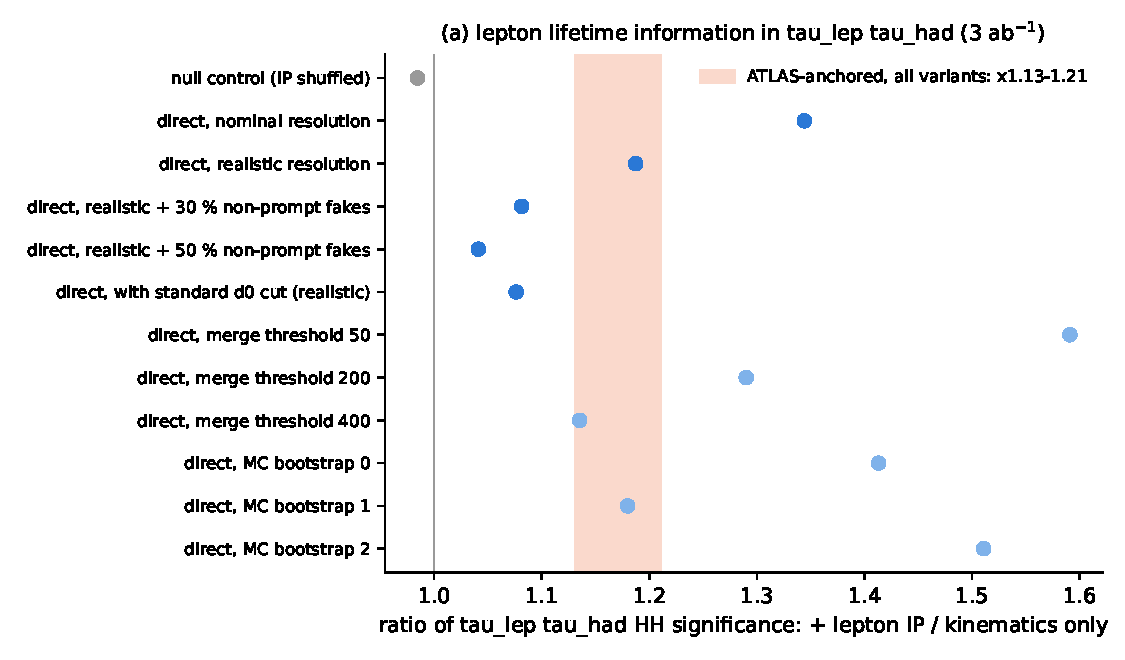
\includegraphics[width=0.75\linewidth]{figures/lephad_ratios.pdf}
  \caption{$\taul\tauh$チャンネルで，レプトンのIPを加えたときの有意度の比．青は直接法の各検証，薄い青はMC統計に関する変種，帯はATLASの組成に固定した因子化法の全変種の範囲．灰色はIPを入れ替えて情報を消した対照．}
  \label{fig:lephad}
\end{figure}

図\ref{fig:lephad}と表\ref{tab:lephad}に結果を示す．まず対照として，真のIPを同じ($p_T$，フレーバー)ビンの中で事象間で入れ替えて起源の情報を消すと，比は$0.98$となり利得は消える．利得がIPの寿命情報から来ていることが確かめられる．

名目の分解能では，直接法の比は$1.34$（$|d_0|/\sigma$だけで$1.37$）である．ビームスポットと$\eta$依存性，電子の裾を入れた現実的な分解能では$1.17$〜$1.19$に下がる．さらにfakeの$30\%$，$50\%$に$b$崩壊型のIPをもたせると$1.08$，$1.04$まで下がる．レプトンに標準の対応づけ要求を課した基準では$1.08$である．直接法の絶対値はビン統合の閾値（50，100，200，400で比$1.59$，$1.34$，$1.29$，$1.14$）や背景MCのブートストラップ（$1.18$〜$1.51$）で大きく揺れ，比の絶対値を決める精度はない．

ATLASの組成に固定した因子化法では，現実的な分解能，IP幅の局外パラメータ，「その他」と非即発fakeの全ての変種で，信号らしさが最も高いビンの比は$1.13$〜$1.21$に収まる（表\ref{tab:lephad}）．本論文ではこれを主たる結果とする．局所基底での3次元のIPは$|d_0|/\sigma$以上の情報を加えず，ハドロン側の偏極の情報（IP・SVを除いたtauspinの入力）の追加は$1.02\pm0.02$で誤差の範囲にとどまる．$\taul\tauh$での利得の正体は，スピンではなく寿命である．

\begin{table}[t]
  \centering
  \caption{$\taul\tauh$の信号らしさが最も高いビンでの，レプトンIPによる有意度の比（ATLASの組成に固定した因子化法，現実的な分解能，IP幅の局外パラメータあり）．}
  \label{tab:lephad}
  \begin{tabular}{llcc}
    \toprule
    「その他」の背景 & fake背景 & SLT & LTT \\
    \midrule
    即発レプトン & 模擬どおり & $1.210$ & $1.182$ \\
    即発レプトン & $50\%$が非即発 & $1.151$ & $1.149$ \\
    即発と$\tau$由来が半々 & 模擬どおり & $1.181$ & $1.162$ \\
    即発と$\tau$由来が半々 & $50\%$が非即発 & $1.132$ & $1.135$ \\
    \bottomrule
  \end{tabular}
\end{table}

\section{HL-LHC投影への換算}\label{sec:proj}

信号らしさが最も高いビンでの比$R_{\mathrm{bin}}$をチャンネル全体へ移すには，そのビン以外の組成を知る必要がある．公開されているのは信号らしさが最も高いビンの組成だけなので，チャンネルの比を
\begin{equation}
  R_{\mathrm{ch}}=\sqrt{f R_{\mathrm{bin}}^2+(1-f)R_{\mathrm{rest}}^2}
\end{equation}
とし，信号らしさが最も高いビンがチャンネルの情報に占める割合$f$を$0.5$〜$1$（Run~2の解析での，そのビンの統計のみの有意度の二乗とチャンネル全体の統計のみの有意度の二乗の比$3.15^2/4.0^2=0.62$を参考値とする），残りのビンの比$R_{\mathrm{rest}}$を1からtopの多い組成での値までとするシナリオ幅で表す．$\taul\tauh$では，即発レプトンの割合が運動学的な領域によらないことから$R_{\mathrm{ch}}\approx R_{\mathrm{bin}}$が期待されるが，下限は$f=0.5$，$R_{\mathrm{rest}}=1$とした．チャンネルを二乗和で結合し，$\bbtt$を$3.1\oplus1.8=3.58$から公表値$3.5$へ比で直し，他のチャンネルを$\sqrt{4.3^2-3.5^2}$とする．ATLAS+CMSは両実験の$\bbtt$に同じ改善が及ぶとして$7.2^2+2(Z_{bb\tau\tau}^2-3.5^2)$とする．

\begin{figure}[t]
  \centering
  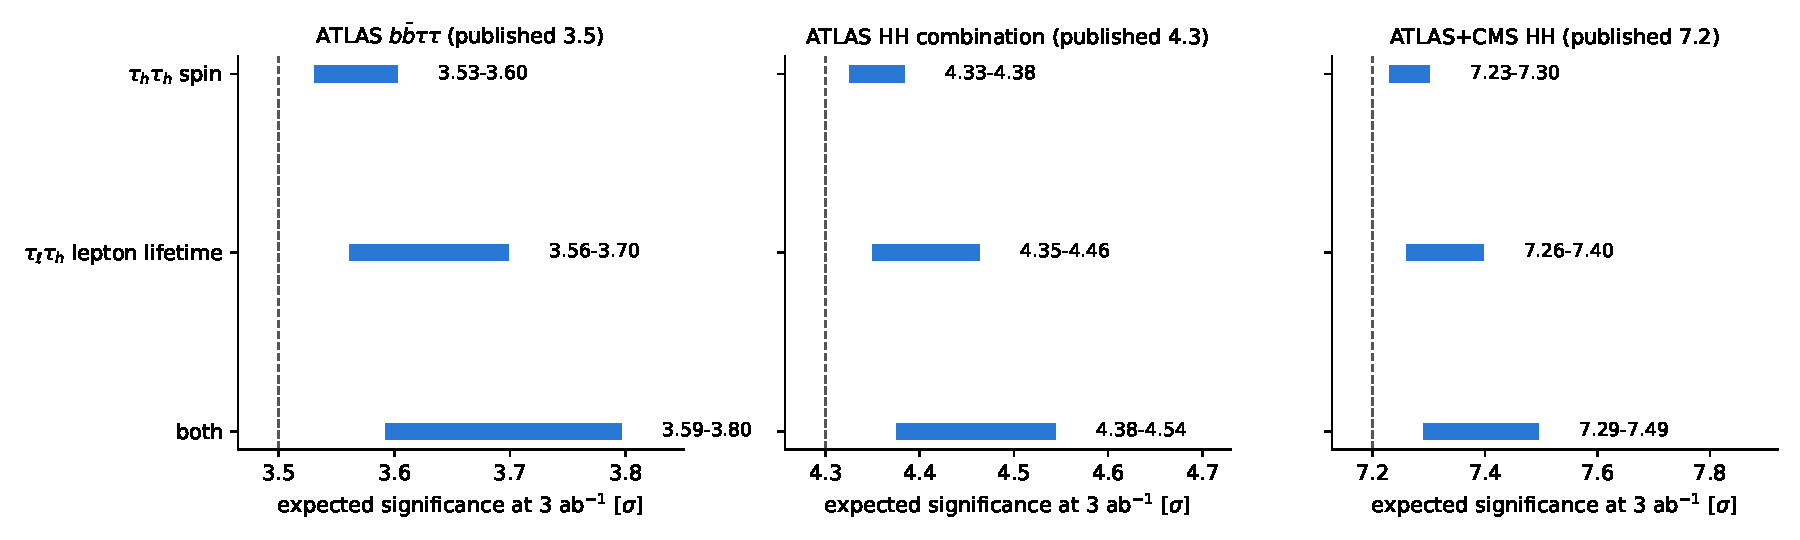
\includegraphics[width=\linewidth]{figures/fig_projection.pdf}
  \caption{$\tau$の情報を加えたときのHL-LHC（$3\abinv$）での期待有意度．帯はシナリオ幅（本文参照）であり，不確かさの区間ではない．破線は公表された投影値．}
  \label{fig:proj}
\end{figure}

\begin{table}[t]
  \centering
  \caption{ATLASのHL-LHC投影への換算（$3\abinv$）．範囲はシナリオ幅．}
  \label{tab:proj}
  \begin{tabular}{lccc}
    \toprule
    加える情報 & ATLAS $\bbtt$ & ATLAS $HH$結合 & ATLAS+CMS \\
    \midrule
    なし（公表値） & $3.5$ & $4.3$ & $7.2$ \\
    $\tauh\tauh$のスピン & $3.53$--$3.60$ & $4.33$--$4.38$ & $7.23$--$7.30$ \\
    $\taul\tauh$のレプトン寿命 & $3.56$--$3.70$ & $4.35$--$4.46$ & $7.26$--$7.40$ \\
    両方 & $3.59$--$3.80$ & $4.38$--$4.54$ & $7.29$--$7.49$ \\
    \bottomrule
  \end{tabular}
\end{table}

結果を表\ref{tab:proj}と図\ref{fig:proj}に示す．両方の情報を加えると，ATLASの$HH$結合は$4.3\sigma$から$4.38$〜$4.54\sigma$（$+2$〜$6\%$），ATLAS+CMSは$7.2\sigma$から$7.29$〜$7.49\sigma$となる．寿命情報の寄与はスピン情報の寄与と同程度かそれより大きい．参考として，非即発レプトンがなく分解能が名目値のままという理想的な場合（$\taul\tauh$で$1.34$倍）には，$\taul\tauh$だけでATLASの結合が$4.58\sigma$になる．

\section{議論}\label{sec:disc}

\paragraph{換算の性格．}本論文の換算は，公開されている信号らしさが最も高いビンの組成と，チャンネルごとの公表有意度から行うシナリオ幅であり，尤度レベルの投影ではない．比$R$は統計と背景規格化（および$\taul\tauh$ではIP幅）の不定性だけを含む尤度で求めており，系統誤差を含む公表値に比をそのまま掛けている．公開尤度を用いれば，信号らしさが最も高いビン以外の組成と系統誤差の相関を入れた，より信頼できる値が得られる．また，投影の元はRun~2のlegacy解析であり，組成に用いた2022年の解析とは解析手法が異なる．

\paragraph{$\tauh\tauh$のスピン．}fake $\tau$はスピン構造なしで代用した．実際のfakeはデータから推定され，回帰器の応答はジェットの構造に依存する．スピン模型の系統は$25\%$の形状の局外パラメータ一本で代表させ，$\pi^0$のエネルギー較正や$\tau$崩壊模型の変動は入れていない．全ての仮説が$HH$の運動学を共有する（因子化）という仮定は，背景MCの統計不足のため実際の$t\bar t$や$Z$の運動学では検証できていない．

\paragraph{$\taul\tauh$の寿命．}最大の不確定要素は三つある．第一は，ATLASの信号領域のレプトンに$d_0$有意度の要求が課されているかどうかである．課されている場合，本論文の模擬ではその要求が$\tau$由来の信号の約$40\%$を落とし，要求ありの運動学のみの有意度は要求なしの約$0.6$〜$0.7$倍になる（分解能の模型による）．したがって，要求を外して寿命で分類することには，本論文の換算よりずっと大きな改善の余地がある．これはATLASの解析の設定で確かめられる．第二は，非即発レプトン（$b$，$c$ハドロンの半レプトン崩壊，光子変換，PVの取り違え）の寄与である．本研究の模擬はこれらを含まず，fakeの一部に$b$崩壊型のIPを与える変種で影響を評価したにとどまる．ATLASのRun~2解析ではfake背景にmultijet由来の成分（非孤立レプトンで定義される非即発レプトン）が含まれており，その割合が利得を左右する．第三は，$d_0$分布の較正である．$R(\tau/\mu)$測定\cite{ATLAS:2020xea}と同様に，$Z\to\mu\mu$や$t\bar t$の対照領域で即発レプトンの分布を較正し，非即発の成分をデータから見積もる必要がある．

\paragraph{IP分解能．}名目の模型にはビームスポットの寄与がなく，楽観的である．現実的な模型で比は$1.34$から$1.17$〜$1.19$へ下がった．HL-LHCの新しい内部飛跡検出器ITk\cite{ATLAS:ITk}は，現行の最内層ピクセル（IBL）より低い$p_T$で分解能が改善すると期待されるが，その効果は評価していない．

\paragraph{tauspinとの関係．}$\taul\tauh$での改善は，tauspinの「PV基準のIPを$\tau$の情報として使う」という発想の延長である．ただし，その中身は偏極ではなく寿命であり，局所基底での3次元表現は$|d_0|/\sigma$以上の情報を加えなかった．スピンの情報が$HH$探索に与える改善は，本論文の範囲では数$\%$にとどまる．

\section{結論}\label{sec:concl}

$\tau$のスピンと寿命の情報が，HL-LHCでの$HH\to\bbtt$探索の期待有意度をどこまで改善するかを見積もった．$\tauh\tauh$チャンネルでは，tauspin水準のスピン情報による信号らしさが最も高いビンの改善は$+2.4\%$であり，背景の大半が単一Higgsと$Z$+HFであるため，偏極計を正確に知っていても$+12.6\%$にとどまる．$\taul\tauh$チャンネルでは，レプトンのPV基準のIPによる$\tau$寿命の情報が，即発レプトンをもつ$t\bar t$，単一top，fake背景を抑え，信号らしさが最も高いビンの有意度を$1.13$〜$1.21$倍に改善する．両者を合わせると，ATLASの$HH$結合の期待有意度は$4.3\sigma$から$4.38$〜$4.54\sigma$，ATLAS+CMSは$7.2\sigma$から$7.29$〜$7.49\sigma$と見込まれる．改善は控えめだが，レプトンの寿命情報は著者らの知る限り既存の$HH$解析で使われていない独立な情報である．信号領域のレプトンに$d_0$有意度の要求が課されているかは確認できていないが，課されている場合にはさらに大きな改善の余地がある．$5\sigma$に向けた$\bbtt$解析の改良として，非即発レプトンのデータによる評価と合わせて検討する価値がある．

\section*{謝辞}
計算にはICEPPの計算機資源を用いた．

\appendix
\section{スピン仮説の密度}\label{app:rho}

本論文で用いたスピン密度（$\tau^-$の偏極計を$\hvec^-$，$\tau^+$を$\hvec^+$とし，局所基底$(n,r,k)$での成分で表す）は次のとおりである．
\begin{align}
  \rho_H &= 1+h^-_nh^+_n+h^-_rh^+_r-h^-_kh^+_k, \\
  \rho_Z &= 1-0.147\,(h^-_k+h^+_k)+h^-_kh^+_k\;\bigl[+0.49\,h^-_nh^+_n-0.46\,h^-_rh^+_r\bigr], \\
  \rho_W &= (1-h^-_k)(1-h^+_k), \qquad \rho_U=1.
\end{align}
角括弧は$Z$の横相関を含める変種である．片側だけ偏極計が定義される事象には周辺密度（$\rho_Z\to1-0.147h_k$，$\rho_W\to1-h_k$，$\rho_H,\rho_U\to1$）を用いた．スピン平坦試料の重みはこれらの値そのものである．

\begin{thebibliography}{99}
\bibitem{Glover:1987nx} E.~W.~N.~Glover and J.~J.~van der Bij, ``Higgs boson pair production via gluon fusion,'' Nucl.\ Phys.\ B \textbf{309} (1988) 282.
\bibitem{Dawson:1998py} S.~Dawson, S.~Dittmaier and M.~Spira, ``Neutral Higgs boson pair production at hadron colliders: QCD corrections,'' Phys.\ Rev.\ D \textbf{58} (1998) 115012, arXiv:hep-ph/9805244.
\bibitem{ATL-PHYS-PUB-2025-018} ATLAS and CMS Collaborations, ``Highlights of the HL-LHC physics projections by ATLAS and CMS,'' ATL-PHYS-PUB-2025-018, arXiv:2504.00672.
\bibitem{ATL-PHYS-PUB-2024-016} ATLAS Collaboration, HL-LHC projection of the $HH\to b\bar b\tau^+\tau^-$ search, ATL-PHYS-PUB-2024-016.
\bibitem{ATLAS:2022xzm} ATLAS Collaboration, ``Search for resonant and non-resonant Higgs boson pair production in the $b\bar b\tau^+\tau^-$ decay channel using 13 TeV $pp$ collision data from the ATLAS detector,'' arXiv:2209.10910.
\bibitem{ATLAS:2020xea} ATLAS Collaboration, ``Test of the universality of $\tau$ and $\mu$ lepton couplings in $W$-boson decays from $t\bar t$ events with the ATLAS detector,'' Nature Phys.\ \textbf{17} (2021) 813, arXiv:2007.14040.
\bibitem{Alwall:2014hca} J.~Alwall \textit{et al.}, ``The automated computation of tree-level and next-to-leading order differential cross sections, and their matching to parton shower simulations,'' JHEP \textbf{07} (2014) 079, arXiv:1405.0301.
\bibitem{Bierlich:2022pfr} C.~Bierlich \textit{et al.}, ``A comprehensive guide to the physics and usage of PYTHIA 8.3,'' SciPost Phys.\ Codeb.\ \textbf{2022} (2022) 8, arXiv:2203.11601.
\bibitem{Elagin:2010aw} A.~Elagin, P.~Murat, A.~Pranko and A.~Safonov, ``A new mass reconstruction technique for resonances decaying to $\tau\tau$,'' Nucl.\ Instrum.\ Meth.\ A \textbf{654} (2011) 481, arXiv:1012.4686.
\bibitem{Cowan:2010js} G.~Cowan, K.~Cranmer, E.~Gross and O.~Vitells, ``Asymptotic formulae for likelihood-based tests of new physics,'' Eur.\ Phys.\ J.\ C \textbf{71} (2011) 1554, arXiv:1007.1727.
\bibitem{ATLAS:ITk} ATLAS Collaboration, ``Technical Design Report for the ATLAS Inner Tracker Pixel Detector,'' CERN-LHCC-2017-021.
\end{thebibliography}

\end{document}
